
\chapter{Generalization Error and Model Selection }\label{ch:modelSelection}

%\section{ Model Selection}\label{section-modelSelection}

In this chapter we will extend some of the Machine Learning concepts introduced in the previous chapter and dive into the different tools that will help us evaluate which are the best models for our task.
These tools will be based on the idea of the generalization error minimization with its descomposition into its bias and variance components.
For our applications, we will settle around model hyperparameter's Cross Validation.
% We will also give a brief mention to the Vapnik-Chervonenkis dimension, as an example of other relevant tools for the discussion.


\section{Prediction and Generalization Error}\label{subsection-generalizationError}

Historically, a convenient loss function used to optimize the model's parameters was to minimize the residual sum of squares.
This measures the performance of our model $f(\cdot)$'s predictions on input samples $x$ with respect to the data's known output classes $y$ as

\begin{equation}
RSS(\theta_0,\cdots ,\theta_p) = \sum_{i=1}^n {[y_i - \hat{y}_i ] }^2 \\
= \sum_{i=1}^n  {[y_i - h( \theta \cdot x_i)] }^2
\label{eq:rss}
\end{equation}

% Yet this loss was favored over other functions because it is more analytically tractable and because of other statistical benefits.
% \begin{equation}\label{eq:rss}
% L(f(x),y) = \left\Vert f(x)-y \right\Vert^2_2
% \end{equation}
% When working with a linear regression with Gaussian residuals, minimizing the residual sum of squares is equal to maximizing the likelihood probability of the target, given the input data.
% This results in minimizing the following sum (RSS):
%Typical of other scenarios such as linear regression, one would like

% The equation reflects our goal to correctly match a training sample with their targets (also known as labels).

We know that the objective is to have a good model in the generlization sense: one which can make a \textit{good} prediction on any sample, even new ones from the true data distribution.
This generalization concept is lacking in the preceding \cref{eq:rss} because it is built to fit the actual dataset in the best possible way.
Given that the training set ($\mathcal{T}$) is a sample of the population, it is not straightforward that the model will perform well accurately any other given sample of the \textit{true} distribution of the data.
%for $\mathcal{T}$.

We need a way of measuring and comparing the generalization power between models to select the best supervised estimator.
For our test data, it means to have a model that can correctly label new samples which were not used in the training phase, such as those from the test set $\mathrm{T_s}$.

% We'll see why it is a bad attempt to generalize the classification model constructed from the data.
% Given that in supervised learning settings, the goal is to build a learner with low predictive error, the algorithm's generalization power will then lie on its ability to

For now, let us assume that $f: X \rightarrow Y$ is a function which represents a true existent relationship in the data such as
$$Y = f(X) + \epsilon$$.

In this mapping from feature to target space we assume $\epsilon$ to be the noise, with a null mean and fixed $\sigma^2$ variance i.e.\ $\epsilon \sim \calN(0,\sigma^2)$.
With this, \cref{eq:rss} can be read as an approximation of the expected prediction error given the training set $\mathcal{T}$.


\begin{definition}{Prediction Error:}
	Given a loss function $L(\cdot,\cdot)$ and a function $f$, we say that the \textbf{prediction error} for the resulting classifier $f$ is
	\[
	PE(f_\theta)= \left[ L(\textbf{Y},f(\textbf{X}))\right]
	\]
\end{definition}

This is the error between our model's output and the target labels, as quantified by the loss function.
 In our specific example, with the parameters $\theta$ encoding the structure of $f$ as $f_\theta(x) = h(x \cdot \theta)$ we would have that:

\begin{definition}{Squared Loss Prediction Error:}
	Given a value for parameter $\theta$ and the \textit{squared error loss}, we say that the \textbf{prediction error} for the resulting classifier $f_\theta$ under the squared loss is

	\begin{equation}
	PE_{true}(\theta) =L(\textbf{y} - h(\textbf{x} \cdot \theta) )  \\
	=  {(\textbf{y} - h(\textbf{x} \cdot \theta) )}^2
	\end{equation}

\end{definition}

Our interest is now in minimizing this error for all possible values from the true distribution, and not only for those in the dataset.
We would like to quantify the expected error over occurrences of $\textbf{X}$ and $\textbf{Y}$ that are independent of $\mathcal{T}$ which is the data used to fit the model.


%This is known as the generalization error and is very related to the prediction error as it is its expectation.

\begin{definition}{Generalization Error}
\begin{equation}
Err = \Expect_{ \textbf{X}, \textbf{Y} } \left[ L(Y,f(X))  | \mathcal{T_s} \right]
\end{equation}
\end{definition}

The problem appears when considering that in this scenario, the models' fit is done on a fixed dataset
and these in turn are a fixed sampled representation of the data.
Thus we are required to estimate the generalization error using only the model's error over the training data that is available.
At the same time we have to ensure that the training and test sets are independent.
%\footnote{In some special scenarios we might have that the data is just constantly incoming and in this way we would definitely have that the data is dynamic. However these are the lesser amount of cases in real applications.}

% $\mathcal{T_s}$:

The generalization error intends to compare the performance of our algorithm trained on a training dataset, with the loss that this model would have had on the true data distribution.
If we consider the case of the squared loss function, we will have that this error now becomes
\begin{equation}
	Err_{\mathcal{T_s}} = \Expect_{\textbf{X},\textbf{Y}} \left[ L(Y,\hat{f}(X)) | \mathcal{T}\right] \\
	= \int_{\mathcal{T_s}} {(y - h(x \cdot \theta) )}^2 P(x,y)dxdy
	\label{eq:squaredGeneralizationError}
\end{equation}

	%\begin{equation}
	%  Err_{true}(\theta) = \Expect[(\textbf{y} - h(\textbf{x} \cdot \theta) )^2] \\
	%  = \int (y - h(x \cdot \theta) )^2 P(x,y)dxdy
	%\end{equation}

\todo{Fix notation mess of $\textbf{X},\textbf{Y}$ vs $X,Y$ and generalization, prediction, EPE, etcs}

Note that in this definition the expectation is taken conditional on the test set and also from which the model is built.

Overall, we are ultimately wanting to know how the learner performs over the true distribution, or what is the average prediction error's for any sample of data.
Note here that we also want to average out any specific influence of the training set on our fit model $\hat{f}$ which was trained from a specific dataset, but also on the $\hat{f^*}$ that would have resulted from training on the true distribution of the data.
With this we can introduce a last definition:
\begin{definition}{Expected Prediction Error}
	\begin{equation}
%	Err = \Expect_{ \textbf{X}, \textbf{Y} } \left[ L(Y,f(X))  | \mathcal{T_s} \right]
	 EPE = \Expect_{X,Y} \left[ L(Y,\hat{f}(X))\right] = \Expect_X \left[  \Expect_{Y | X} \left[   L(Y,f(X))  \right]  \right]
	\end{equation}
\end{definition}

%\begin{equation}
% \end{equation}.

In practice we have finite access to samples, so we have to estimate the expected prediction error by means of the generalization error.
From the data, we will build or \textit{train} our model and from this reduced sample we will extract a training error to determine how well the model is performing.

This will be our approximated $EPE$ through the

\begin{definition}{Training Error:}
	is the average loss over the sample prediction errors:
	$$ \overline{err}_{\mathcal{T}} = \frac{1}{N} \sum_{i=1}^N L(y_i, \hat{f}(x_i) )$$
\end{definition}\label{def:trainingError}

%Let \textbf{x} $\in \mathbb{R}^{p}$ denote a random input variable and \textbf{y} $\in \mathbb{R}$ denote a random output variable with joint distribution $P\left(\textbf{x},\textbf{y}\right)$.

In order to find the best model for our task, we will turn to rank different ones according to their training errors over $\mathcal{T}$ and $\mathcal{T_s}$.
Combinations of high or low values for these, across training and test data, will be used as model evaluation and by this we will start to find aspects of the algorithm which need improvement.

\section{Bias and Variance}\label{section-biasVariance}

If we look closer at the $EPE$ for the specific case of the squared loss function with

\begin{equation}\label{squaredPE}
EPE = \Expect_X \Expect_{Y|X} \left[ \left\Vert Y - \hat{f}(X) \right\Vert_2^2 \right]
\end{equation}

It is not difficult to see that the model that minimizes this error is
$$\hat{f}(x) = \Expect \left[ Y | X=x \right] $$
We say that our model $\hat{f}$ is an estimate of the true relation in the data, and takes the form above, with the form structure from the data.

With the squared loss, the expected prediction error
$$\Expect \left[ \left\Vert Y - \hat{f}(X) \right\Vert_2^2 \right]$$
of the model can be decomposed in the following way:

\begin{equation}\label{squaredBiasDecomposition}
\begin{split}
EPE( \hat{f} ) = & {\Expect_X \left[  f(X) - \hat{f}(X) \right]}^2 + \Expect_X \left[ {\hat{f}(X)}^2 \right] \\
& - {\Expect_X \left[ \hat{f}(X) \right] }^2 + \sigma^2 \\
= & {Bias(\hat{f})}^2 + Var(\hat{f}) + \sigma^2
\end{split}
%= Bias(\hat{f})^2 + Var(\hat{f}) + \sigma^2
\end{equation}


 \cref{squaredBiasDecomposition} is hereby refered to as the \textit{bias-variance decomposition for the squared loss} where the first term is called the square of the estimator's bias.
This measures how good are our estimator's predictions compared to the true relational function.
The second and third terms are the estimator's variance.
This will measure how this random variable varies along its most expected value.
The noise's variance term is that part of the prediction error which is irreducible.
Note that we have already taken the expectation over the target and that is why we are left with the target's inherent noise.
This part of the error we cannot reduce or control with our learner model since it is caused by the problem's random nature.

In the $EPE$'s decomposition we are integrating over the joint distribution of inputs and outputs.
As we've mentioned before, we have incomplete information on $P(x,y)$ given the limited amount of information in $\mathcal{T}$.
We must assume then that calculating this integral is not possible for any $\theta$ so we must rely on estimation procedures.

For example, we could try and sample $M$ i.i.d.\ points from $P(x,y)$ to approximate the integral by a Monte Carlo scheme.
With the squared loss function this would look as

\todo{Confusing notation with epe, prediction, err_true, etc}
\begin{equation}\label{eq:mcarlo-approx}
Err_{true}(\theta) \approx \frac{1}{M} \sum_i^M {( y - h(x \cdot \theta) )}^2
\end{equation}

Yet this would be unfeasible as well for all of our possible $f( \theta)$ models since the sampling process should be done for each specific $\theta$.
%Notice however the close resemblance of the \cref{eq:mcarlo-approx} to the form in \cref{eq:rss}.

Historically, the concepts of bias and variance where associated directly with the squared loss function and in the literature it is said that algorithms have ways of attacking these two sources of error.
They are key elements in the expected prediction error and they point to different weak spots in the algorithms.
At the same time, different methods are used to improve each of them, where ultimately our having control over both errors is central to our prediction task.
Authors point that in practice it is usual that the improvement of one generally leads to a decrease in the other.

%For this, we use a simple series approximation
%
%\begin{equation}
%Err_{train}(\theta) \approx  \Expect_{ \mathcal{T}}[{(y - h(x \cdot \theta) )}^2]
%\end{equation}

%, and can be decomposed into two types of errors


Conceptually the bias error represents the model's accuracy in labeling predictions correctly.
It is the model's best attempt to capture the functional relationship among the feature and target variables.
This could either mean it is correctly assigning the sample to its correct class in classification settings, or, in a regression setting, by estimating a value for that sample which is \textit{near} to the target value.

The bias is lower when models correctly learn the underlying structures of the data.
However, as bias decreases, the model complexity increases and more data is needed to train it correctly because the model becomes very fit to the training set i.e.\ it loses the ability to extend this predictive accuracy to new samples because the model learns too much from the available samples only.
In this situation, we have another type of error which is when we have an increase in variance.

%In the generalization error, the loss function determines how \textit{good} the model's prediction are by quantifying these errors.
%We can extend the notion of bias and variance to loss functions more general than the squared loss error.
%Given a training set $\mathcal{T} = (X,Y)$, let $\hat{f}(X)$ be the model's predictive function for the features and denote $L( Y,\hat{f(X)} )$ the loss function acting on the data.


%We will denote $K = |\calG|$ as the number of classes.
In classification problems it is uncommon to use the residual sum of squares to fit the model's parameters and there are other \textit{loss} functions to rely on.
Specifically in the binary classification context, a common loss function used is

\begin{equation}
L(Y, \hat{f}(X)) = I(Y \neq \hat{f}(X))
\end{equation}\label{eq:classificationLossFunction}

where $Y$ will be taking any of value of the class set $\calG$.
%$$.
% In multi-class supervised problem setting,

With this loss function, the classification prediction error can be decomposed in

% \begin{equation}

%$$
%EPE( \hat{f} ) = P\left( \hat{Y} \neq Y \right) = Var(Y) + P\left(Y=\argmax_{1\leq i \leq K} P(\hat{f}(X) =i )\right) -
%\sum_{i=1}^K P(\hat{f}(X) =i)P(Y=i) $$

% \end{equation}
% \begin{split}

%EPE( \hat{f} ) =
% using equation numbers from James'  paper (N)
$$
P\left( \hat{f}(X) \neq Y \right) =
Var(Y) + % (19)
P\left( Y =  \argmax_{1\leq i \leq K} P(\hat Y = i ) \right) % (22)
%P\left( Y = \argmax_{1\leq i \leq K} P(\hat{f}(X) = i ) \right)  % part of AE (21)
-  \sum_{i=1}^K P(\hat{f}(X) =i)P(Y=i) %  AE (21)
$$

where in this formula we have, once again, that the error is decomposed by using the classifier's variance. 
Here, the classifier's bias is not clearly defined as with the squared error.
Yet the decomposition quantifies how similar is the learner's class probabilities with the true distribution in the data, and how this interaction differs from the most probable output value, which is the Bayes classifier.

Note that in this definition we do not have the bias of the model as a term of the error.
This quantity is rather taking effect as part of the second and third summands in the equation and it tries to capture how close is the classifier's distribution with respect to this distribution in the data.
Another relevant difference is that in this definition there are no noise terms 
For more detailed information on bias and variance decomposition in classifiers, one can refer to \cref{appx:sec:biasVarianceExtensionLoss} which is based on the survey work of~\citep{james-biasVarianceGeneral}.

%What is also interesting to note with this formula is that it might be that due to the interaction in between target and model probabilities, we have that in some cases we might have in

\subsection{Overfitting}\label{subsection-overfitting}

For any given Machine Learning learner, we can have different combinations of high or low variance and biases.
Naturally that makes three cases out of four model performance scenarios that need to be improved, where we have low bias and/or low variance.
For each combination of bias and variance stages, there are different strategies to improve a model.
For example, in one of the most common scenarios we might have a model that has a high overall variance and low bias.
If we also have that the model has a good performance on $\mathcal{T}$, whilst having a poor performance on $\mathcal{Ts}$, it is said in the literature that the model is \textit{overfitting} the data.
The reasons behind this scenario can be various and most of them are related to learners which are overly-complex or situations in which there is insufficient training data.
This results in learners which are only suited for the training set.

% For each case there are distinct strategies we can apply to improve the model.
% We will have to work the data better and find ways to tune the model itself in order to improve one or another type of error.
 % we will need to determine how to improve our model
 % to work out the data and tune the model to lower both errors.

Overfit models will also fail to generalize on new data since the variance structure of the training set is such that the number of training samples is not enough to lower the overall variance of this model.
To illustrate this point, in \cref{figure:dtree_overfit_problem_2} we show the results from fitting a learner on our own CDR dataset.
We fit a Decision Tree classifier on \cref{target2} which has a high imbalance between the positive and negative target classes to illustrate the interaction between bias and variance.
A discussion of this model's formulation is presented in \cref{ch:ensembleMethods}.
This is a tree based model which increases its complexity by growing the tree's depth.
In turn, this increases the number of features used in by the leaner to decide on the predicted target.

% A learner with of this characteristic will only work very accurately on the train set with poor performance on new samples.
%Here we use , to try and produce a model which overfits $\mathcal{T}$.

%It is clear here that higher depth implies increasing model complexity\footnote{A detailed explanation of this technique can be found later in \cref{section:decision_trees}.}.

To measure the performance of the fit learner, we take a scoring function for the model's performance which outputs a value in the range of $(0,1)$. With this functino we have that higher values means better scores.
We will introduce later specific formulations for scores generally used.
In this way, \cref{figure:dtree_overfit_problem_2} graphs how the model performs at different levels of model complexity.
In the image, the test and training errors are given as a function of the tree's depth.

%This is because Curing the optimization procedure, the algorithm has to fit more parameters.
%In this sense, the model increases in complexity, as measured in its degrees of freedom.

\begin{figure}[h!]
\begin{center}
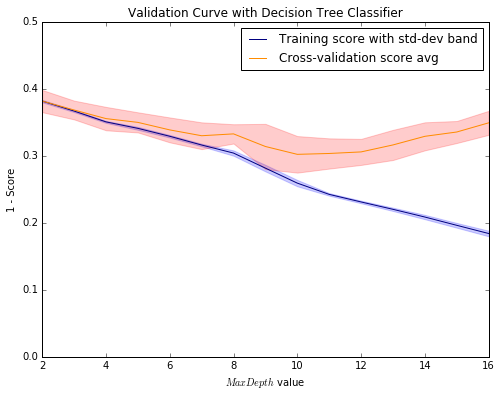
\includegraphics[width=1\columnwidth]{figures/figure-biasVariance/dtree_overfit_problem_2.png}
\caption{ Training and cross-validated mean $Accuracy$ score functions along the change in max tree depth.
For \cref{target2}, one model is fit for each tree depth value on both the training and cross validation sets.
Both score series are compared side by side, with their corresponding standard deviation band for the CV folds.}
\label{figure:dtree_overfit_problem_2}
\end{center}
\end{figure}


At first the model's bias is high both for the training and testing sets, and as a consequence, we would expect to have a high generalization error.
We later see how the overall error decreases as complexity increases.

An estimate of the expected prediction error is shown, calculated by averaging over the test set' prediction error's.
We note how at first it decreases when the model's complexity is increased.
However, later when the model starts to overfit the data, we can see how the test error starts to rise whilst the train error keeps decreasing.
This situation is important to our $EPE$ estimation cause it hints that the model has lost predictive power due to an increase in variance.

In \protect\citep{hastie-elemstatslearn} the authors give a rough heuristic to select the best model: stop increasing the model's complexity once the estimated $EPE$ stops decreasing.
That is, chose the point where the scoring error of the test set stops decreasing along with the training error.
For \cref{figure:dtree_overfit_problem_2}, this would roughly be when $Max Depth = 10$.

In this example we are only looking for the best model over a search space of one dimension, namely the tree-depth hyperparameter only.
In practice, the models will have more parameters to tune and this makes finding the lowest prediction error for all possible models difficult.
Still, we might settle for near-optimal models which reach acceptable error scores.
The following section introduces the assumptions to consider the test error as a good approximation of the generalization error.
It also gives a formal argument in favor of finding models whose scores are not optimal for that dataset.


\section{Cross Validation (CV)}\label{section:crossValidation}

Classification models are algorithms which intend to build approximating functions to a stochastic process, by means of algorithms.
Due to the searching nature of this process, in the generally large space of hyper-parameters, we have that when models are fitted, we ultimately create different learners.

These differences between learners are controlled by the \textit{parameters} or configuration of the algorithm.
And the nature of each parameter can be due to reasons such as computational or statistical  algorithmic variants.
An example of this, which was introduced in \cref{section-hyperParametersRegularization}, is the $\lambda$ penalization parameter in a Logistic Regression.
In this case we have that $\lambda$ controls the amount of weight to be placed on the regularization term of the minimized function.


Under this setting Cross Validation (CV) is a technique introduced to systematically explore tuning parameters values and decide which learner is better for the task at hand.
It intends to help in provide a better way of estimating the $EPE$ during the process of finding the best hyperparameters.

By comparing the generalization error of each model, where models vary accordingly with the hyper-parameters' values, the model's evaluation score is used to select the \textit{best} model in the class.

The technique is the most widespread for evaluating the generalization performance of a set of learners.
Given a number of possible configurations or values for the tuning (hyper) parameters of an algorithm, we would want to decide which selection of these fit the best estimator $\hat{f}$, as measured by the generalization error.

%
%In terms of the concepts introduced before, the quality of an estimated model  from a family of algorithms is evaluated in the Cross Validation procedure.
%Where quality refers to the rate of generalization error.

In most problems we will have that data is scarce and, at the same time, we have that prediction error estimates are hardly computable in practice.
In part, this because estimates are based on assumptions that are not practical: they rely on the true distribution of the data, access to an \textit{infinite} amount of data, or because they are based on analytical results which are difficult to compute.
To cope with this, CV intends to prevent over-fitting problems and improve the $EPE$ estimation procedure by applying a procedure which iteratively holds out a random split of the dataset.
With this, the procedure will measure the predictive accuracy of the learner fit of data \textit{in-sample} against values from the \textit{hold-out} part of the dataset.
In a sense, hold-out samples are acting as ``test''  to the learner fit with in-sample data.
As usual, the evaluation measure here is given by the loss function, which we must select beforehand.

\subsection{Formulation of the Cross Validation (CV) Procedure}\label{subsection:crossValidationProcedure}

In this method, we will denote a partition of the samples as a \textit{fold}.
CV will then partition the data into $K$ random separate \textit{folds}, where the number $K$ is preset\footnote{ We assume here that we are selecting samples from the training set $\mathcal{T}$ and not from the test set $\mathcal{T_s}$.}.

Let $\gamma : \{1,\cdots ,N\} \mapsto \{1, \cdots , K\}$ be a function mapping samples to folds.
Without loss of generality, let $\alpha$ be an index of the model's hyper-parameters configurations, where each distinct value combinations for all tuning parameters is identified by this index\footnote{ Note that the domain of $\alpha$ will vary with each model, which defines the type of algorithm used to learn.}.

The idea behind the CV algorithm is to run an iteration over all the folds, denoting $k \in [1,\ldots,K]$ the iteration indexer.
It will then take one fold $\gamma^{-1}(\{k\})$ to be the validation set and if we let $\hat{f}^{-k}$ be the fitted estimator on the training set and $k$-fold hold out, the classification performance will be tested against these \textit{out of sample} estimates.
Finally we will have that for every sample in this $k$-fold, we will measure the loss $L(y_i, \hat{f}^{-\gamma(i)}(x_i))$ of the in-sample model's prediction, against the true target's value.
The average score over all samples would get us the Cross Validation error for this problem instance.

We see that Cross Validation intends to estimate the expected \textit{out-of-sample} error $\Expect \left[ L(Y, \hat{f}(X)) \right]$, when the model is tested against \textbf{independent} samples from the true distribution.
To do this it is fundamental to ensure independence of the training set and the test set.
Any data transformations that must be done on the input data $X$ that jointly uses the output samples $Y$ in the process, must be done or ``learned'' only on the training set.
It is important that no information from our test set is introduced into the final estimator output from the CV procedure.

Models have to be agnostic to any information contained in $\mathcal{T_s}$.
In a sense this means that the learner never ``sees'' any test data until we use it to evaluate our learner's performance.


\subsection{Selection of tuning-parameters (hyper-parameters) }\label{subsection:selection_hyper_params}

The CV procedure provides a reliable $EPE$ estimate to select the best values for the algorithm's tuning parameters.
These hyperparameter configuration will be \textit{best} in the measure provided by the loss funciton.
Let $\mathcal{A} = [\alpha_0, \alpha_1,\ldots, \alpha_l  ]$ be a list of hyperparameter settings and $\mathcal{K} =[1,\cdots ,K]$ a list of folds.
To clearly depict how a full K-Fold Cross Validation procedure runs, we outline its pseudo-code.

 \begin{algorithm}[H]
 \KwData{All hyper-parameter configurations $\mathcal{A} = [\alpha_0, \alpha_1,\ldots, \alpha_l]$ and a number $K$ of folds.}
 \SetAlgoLined\KwResult{Data table mapping error scores to hyper-parameter configurations $CV(\alpha) \ \forall \alpha \in \mathcal{A} $}
 Initialize $\mathcal{A}$ and $\gamma(\cdot)$\;
 \For{ $\alpha \in \mathcal{A}$}{
 \If{data transformation}{
 Perform data transformation on the whole training set $\mathcal{T}$ \;
									 }
 \For{ $k \in \mathcal{K}$}{
 	 \If{feature selection}{
 	 	Perform feature selection on the $\textrm(T)^{-k}$ \;
 	 }
 fit $\hat{f}^{-k}(\cdot, \alpha)$\;
										}
 compute $CV(\alpha) = \frac{1}{N} \sum^n_{i=1} L\left( y_i, \hat{f}^{-\gamma(i)}(x_i, \alpha) \right)$\;
												}
 \caption{Pseudo-code for K-Fold Cross Validation Estimation for an index of $\alpha$ hyper parameters.}
 \end{algorithm}

Note that during the loop for $\alpha$, each sample's prediction is tested on the model which was fitted without using that same sample.
This is central to the idea of cross-validation in which training samples are used \textit{as if} they were testing samples.
%Samples that are not used to train the model in the CV procedure are called validation samples.

With this method, it makes sense to choose a final model $\hat{f}_\alpha$ with the lowest $CV(\alpha)$ score among all possible hyper-parameters.
However, following ideas detailed in \cref{appx:sec:vcDimension}, importance should also be given to the \textit{complexity} of the approximating function.
A common rule of thumb is to favor models in which we use a lower number of hyper parameters or features.
In practice however, a class of approximating functions might have a defined complexity which is not analytically computable.
Thus in some cases, crude heuristic estimates or common sense is used to estimate model complexity, without making use of theoretical arguments.


\subsection{CV run on CDR data}\label{subsection:cvExperiment}

As an example, we consider here a cross validation procedure over a Logistic Regression model.
Here we are using \cref{target2} which is defined to find those users that used to live in the endemic area and eventually migrated out of it, becoming non-endemic during the training phase.
This procedure serves as a benchmark to compare different hyperparameter configurations.

In this case we decide to optimize the model's regularization strengt which is captured in the parameter $C = \frac{1}{\lambda}$.
Recall from \cref{eq:logitRegularization} that this is the regularization strength of the model, and note that a smaller value in $C$ is a stronger regularization.
We perform this experiment and consider the difference in scores between  $\mathcal{T}$ and $\mathcal{T_s}$ for each possible $C$ value.
It is important to note that all test scores were performed on models built only from $\mathcal{T}$.

\begin{figure}[h!]
\begin{center}
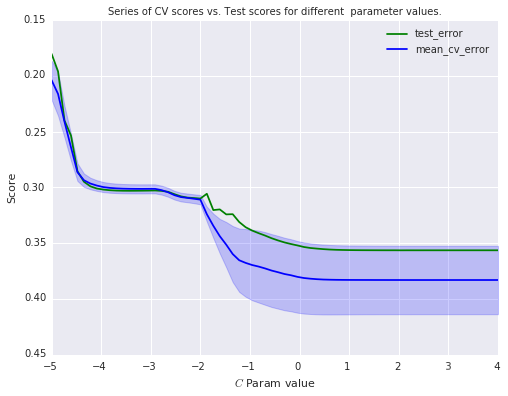
\includegraphics[width=1\columnwidth]{figures/cross_validation/train_and_cv_score_comparison_logreg.jpg}
\caption{ Comparison of 12-fold cross validated and test average errors for \cref{target2}. Negative log loss ($NLL$)a scores are shown for each value of the regularization parameter $C$. Standard deviation bands on the $K$ fold errors are added to the CV series.}
\label{fig:cv_vs_test_score}
\end{center}
\end{figure}

In \cref{fig:cv_vs_test_score} the x-axis represents the parameter $C$'s shown on a $\log_{10}$ scale.
The score used is the negative log loss function on a twelve fold cross validation set.
Both the training and the mean cross validation scores are shown.
% In parallel to this we have scores over the test set.

It is interesting to see that for low $C$ values, the test and CV scores are very similar in that they have are better scored.
This is probably due to the fact that being on a log scale, the algorithm's regularization dominates the optimization routine.

However, at some point near $\exp(-2)$, both lines separate differ in a notorious way.
This continues to be notorious in the direction of increasing $C$ values.
Here it can be seen that the test score is barely in the one standard deviation band of the average CV score.
This image serves as an example of how different the CV and test scores can be.

With this we have come to show an example of how Cross Validation approximates the test error of a model.
The method required only minimal information from the data to do this, yet we have to preset a value for the number of $K$ folds to use.

To determine this value a priori might not be possible and experimental results in the literature show the different results for CV routines with varying $K$ number of folds.
For more information on this please refer to \cref{appx:sec:optimalKfoldNumber}.


\subsection{CV Scores in Classification Learning}\label{section:scoring_functions}

In binary classification, the contingency table is a good tool to summarize a learner's training performance over samples in $\mathcal{T}$.

Let $\hat{f}$ be our model learned from the data after a CV procedure.
To construct this table we note that for each sample, there can only be four possibilities when comparing the model's prediction and the sample's observed target value.
The contingency table then shows the count of samples that fall into each of the these four groups.
% Every sample has a target value $y$ and a predicted outcome $\hat{y}$ and there are only four possible interactions of these two variables, for two binary outcomes each.

We can express the models' target value $\hat{y}$ into the positive ($\hat{P}$) or negative ($\hat{N}$) categories.
At the same time we can set actual target data into the positive ($P$) or negative ($N$) categories.

To assess the performance of the classification algorithm and pick the \textit{best} model we must decide on how the CV procedure will value two different models.
For this we must evaluate the mismatch between the target and the predicted value in a quantifiable way.

In this context these evaluating functions are also known as \textit{scores} or \textit{measures} and they are built by looking at how many times an algorithm misclassified instances, and in which situations do the misclassification happen.
To visualize this, the \textit{confusion} table presents these results in the following table:

\noindent
\renewcommand\arraystretch{1.5}
\setlength\tabcolsep{0pt}
\begin{tabular}{c >{\bfseries}r @{\hspace{0.7em}}c @{\hspace{0.4em}}c @{\hspace{0.7em}}l}
\multirow{10}{*}{\parbox{1.1cm}{\bfseries\raggedleft\ Target\\ value $y$}} &
& \multicolumn{2}{c}{\bfseries Predictive value $\hat{y}$} & \\
& & \bfseries \^{P} \ $(0)$ & \bfseries \^{N} \ $(1)$  \\
& P \ $(0)$ & \MyBox{True}{Positive (TP)} & \MyBox{False}{Negative (FN)} & \\[2.4em]
& N \ $(1)$ & \MyBox{False}{Positive (FP)} & \MyBox{True}{Negative (TN)} & \\
%& total & P \ $(0)$ & &
\end{tabular}

\medskip

These cell values count the amount of instances that fall into each of the four possible outcomes.
Building from this, we have metric scores constructed to provide values on the algorithm's performance.
These counts are combined in different transformations that measure different aspects of an algorithm's classification performance.

Some of the most common metrics include the following:

\begin{itemize}
\item \textbf{True Positive Rate (Recall):} $\frac{TP}{P} = \frac{TP}{TP + FN}$ \\ This rate measures the percentage of real positive values captured by the algorithm.
A high recall of the algorithm indicates that a high number of the real positive labels were classified as positive.


\item \textbf{Positive Predictive Value (Precision):} $\frac{TP}{\hat{P}} = \frac{TP}{TP + FP}$ \\ This rate measures the \textit{confidence} of the algorithm in its predictions of the positive class, where a high precision indicates value in its predictions.

\item \textbf{True Negative Rate (Specificity):} $ SPC = \frac{TN}{N} = \frac{TN}{TN + FP}$ \\ This rate measures the percentage of real negative values captured by the algorithm.


\item \textbf{False Positive Rate (Fall-Out):} $FPR = 1 - SPC$ \\ This rate measures the percentage of false negative values misclassified by the algorithm.

\item \textbf{Accuracy:} $\frac{TP + TN}{P + N} = \frac{TP + TN}{TP + FP + TN + FN}$ \\ This rate measures the \textit{confidence} of the algorithm in all of its predictions.


\item \textbf{F1 Score:} $\frac{TP + TN}{P + N} = \frac{TP}{TP + FP} = 2 \frac{1}{ \frac{1}{recall} + \frac{1}{precision} }$ \\ This is the harmonic mean of the recall and the precision metrics.\@ It's advantage is that it can capture both of the scores with equal weight.
Its values range in the ${[0,1 ]}$ domain and are ordered in the sense that perfect classifiers have an $F1$ score of 1.

\end{itemize}


To illustrate the difference in these metrics we ran an experiment on \cref{target2} where we intend to correctly classify users that moved out of the endemic region from the past to the current time period.
We took one logistic classifier with common settings and we ran a cross validation procedure over values of the regularization strength $C$.

In this run, we considered four metrics to cross-validate our models: $Accuracy$, $Precision$, $Recall$ and $F1$.
We compared all of them in a procedure which had fixed hyper parameters for all models.
The number of folds, $K$, was set to eight and the lasso regularization ($l1$) configuration was optimized.
At the same time, we fixed to $100$ the maximum gradient descent iterations for every configuration tested.
We also balanced the contribution of the positive and negative samples to the loss function, where samples of the , under-represented, positive class had a higher contribution to the loss.
This was done by reweighting each individual sample's loss, where the weight was equivalent to the reciprocal of that sample's class percentage with respect to the total number of samples.

For each metric, the best model output from the CV procedure which was selected based on the score.
All winning models were then evaluated against $\mathcal{T_s}$ to give a final evaluation metric on the model's performance.
No other information from $\mathcal{T_s}$ was used during the whole process.
In \cref{tab:metrics_comparison_logreg_target1_results} we show a summary of these benchmarks.


\begin{table}[!htb]
\caption{ Results comparing an 8-fold CV on \cref{target2}, using a Logistic Classifier over varying regularization $C$ values.
Four metrics were cross-validated and compared in this experiment: $Accuracy$, $Precision$, $Recall$ and $F1$.}
\label{tab:metrics_comparison_logreg_target1_results}
\centering
\begin{tabular*}{0.9\textwidth}{@{\extracolsep{\fill} }  l l l l l }
%{|p{2cm}|p{2cm}|p{1.5cm}|p{1cm}|p{1.5cm}}
\toprule
Metric & Best $C$ value & Mean CV score & Test score & Full CV time (s)  \\
\midrule
$Accuracy$ & 0.316 & 0.685 & 0.695 & 4628.3  \\
$Recall$ & 0.107 & 0.637 & 0.612 & 4638.2 \\
$Precision$ & 0.0006 & 0.038 & 0.035 & 4667.5 \\
$F1$ & 0.0015 & 0.0071 & 0.005 & 4612.1 \\
\bottomrule
\end{tabular*}
\end{table}

It is clear from these results that all metrics favor strongly regularized models, except for the $Accuracy$ metric which favored the least regularized models of all CV procedures.
As expected, calculating each score is straightforward from the contingency matrix and there are no significant runtime differences among them.
CV procedures all take nearly the same time to compute.
%that there are no significant time differences in choosing one metric over another.

Among all best-fit models, the biggest difference in test and average CV scores was of $4\%$, yet the algorithm had very poor performance when finding samples of the positive class.
This is evidenced in the extremely low value for the $Precision$ scores where only a handful of positive classes can be correctly captured by the model.
The effect of the low precision is also evident in the $F1$ score which drags this metric to extremely poor levels, even when the $Recall$ had an acceptable rate of 0.65.
This is a strong indicator of a very ill-conditioned problem, where the class imbalance strongly affects the detection of positive cases over all positive predictions made.
For this case, the positive class samples were less than $1\%$ of all samples.

% Keeping all of the above in mind, in practice an experimenter would chose a metric which is domain specific and appropriate for the task at hand.
% The quality of solutions will then vary with the way they are evaluated, and this evaluation will depend on the task itself.

\subsection{ROC Curve}\label{sub:roc_curve}

One last important metric that is generally used in classification tasks is one related to the ``Receiver Operating Characteristic'' (ROC) curve.
The metric itself is a measure of the \textbf{Area under ROC curve} ($ROC AUC$) and it applies only to algorithms which output for each sample the probability of belonging to the positive class.

With these algorithms we would have that the output label will be defined as

\begin{equation}
\hat{y} =
\begin{cases}
&1 \ \mbox{if} \ f(x) > \pi \\
&0 \ \mbox{else}.
\end{cases}
\end{equation}

where $\pi$ is a threshold value which will set the algorithm's decision level, that which separates positive from negative samples.

If we consider different values for $\pi$, we will see that the true-positive rate $TPR$, or recall, and the fall-out $FPR$ of the algorithm will vary depending on this confidence level $\pi$.
With this, we can define the ROC curve to be

\begin{equation}
\sigma(\pi) = (R_\pi, FPR_\pi)
\end{equation}

As expected, there exists a functional relationship between these two as the threshold is varied.
The image of $\sigma(\cdot)$ is a curve defined in $[0,1]\times[0,1]$ which is referred to as the \textit{ROC space}.

To find a balance between these two rates, the $ROC AUC$ metric measures the integral of this curve in ROC space.
The score calculated is thus known as \textit{Area Under the ROC Curve}.

This metric follows the same properties as the ones mentioned before, where the best classifiers have values closer to $1$.\footnote{As a side note, the $ROC AUC$ measure is proportional to the statistic of the Mann-Whitney U-test, where the classifier's mean output positive and negative classes are compared.
More information on this can be found in \citep{mason-rocAucRelationship}.}

The following figures are example ROC curves for two of the problems defined from our dataset.


\begin{figure}[h!]
\begin{center}
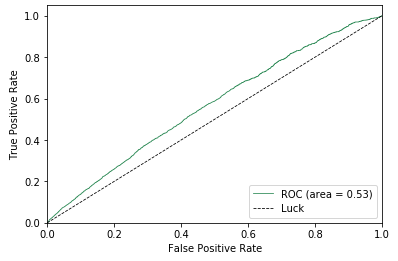
\includegraphics[width=1\columnwidth]{figures/figure-lowROCAUC/figure-lowROCAUC_original}
\caption{Example of a ROC curve from a Decision Tree classifier used on \cref{target2}. A 8-fold CV procedure is fit and then the best learner's performance is evaluated on $\mathcal{T_s}$ which gives score of $0.53$. This model was specifically built to overfit the dataset by constructing a tree of 12 levels.}
\label{fg:lowROCAUC}
\end{center}
\end{figure}

Notice the algorithm's poor prediction performance where the $ROC AUC$ output is near to the `random' line.
This line constitutes the performance of a \textit{random} classifier which arbitrarily labels samples as being to each possible class.
Under normal cirumstances we expect to construct learners that have better $ROC AUC$ scores than a \textit{random classifier}.
To do this fit, we configured the Tree's hyperparameters with a bad nature and, in effect, this outputs a learner which has a poor performance in the training error.
% a very limited search over the Tree's hyper-parameters.


As another example, the same algorithm was run but on \cref{target1} and using the same available data as in \cref{fg:lowROCAUC}.
For this problem we are looking for those useres that had lived in the endemic region in the past regardless of their current endemic situation.
This problem does not suffer from class imbalance, where the positive class constitutes $30\%$ of all samples.
In \cref{fg:highROCAUC} we show a similar figure as in \cref{fg:lowROCAUC} to illustrate the difference ``ROC'' curves that result from this optimization.

\begin{figure}[h!]
\begin{center}
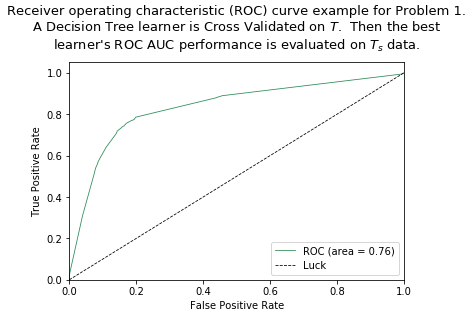
\includegraphics[width=1\columnwidth]{figures/figure-highROCAUC/figure-highROCAUC}
\caption{Example of a ROC curve from a Decision Tree classifier used on \cref{target1}. An 8-fold CV procedure is fit and then the best learner's performance is evaluated on $\mathcal{T_s}$ which gives score of $0.76$.}
\label{fg:highROCAUC}
\end{center}
\end{figure}

The results in this case is that the algorithm has a considerable better score by the $ROC AUC$ metric.
No data transformation has been applied to the dataset between runs.
The difference in the two scores is notable and corresponds entirely to the problem chosen.

\subsection{Final experiments on model selection}\label{sub:final_model_selection}

As a last remark for this chapter, we show here a brief experiment with a Logistic Regression Classifier.
In this, we explore different hyperparameter configurations over a full CV procedure.

The idea is to predict which users lived in endemic regions in the past (again this is \cref{target1}), yet excluding the feature that indicates in which state the user is currently living.
We also set the ``ROC AUC'' metric to compare the $l1$ vs the $l2$ regularization of the model on more than a hundred values for the regularization parameter $C$.

For both regularization types, we set a value for $C$ that ranged from $\exp(-2)$ to $\exp(5)$.
Over all, we implement a cross validation routine of 8-folds.

\cref{tab:roc_auc_logreg_target1_results} shows a summary of results.
In these, our experiments resulted in higher values for $l1$ regularized models.
This gap is gets wider when comparing test scores for both and the same happens to the time taken to fit the cross validation algorithm for all of the $C$ values.

\begin{table}[!htb]
\caption{Table of results comparing an 8 fold cross validation fit for a Logistic Classifier with varying regularization $C$ values for \cref{target1}.
The metric for this experiment was the ``ROC AUC''.}
\label{tab:roc_auc_logreg_target1_results}
\centering
\begin{tabular*}{0.9\textwidth}{@{\extracolsep{\fill} }  l l l l l }
%{|p{2cm}|p{2cm}|p{1.5cm}|p{1cm}|p{1.5cm}}
\toprule
Regularization type & Best CV $C$ value & Mean CV score & Test score & Full CV time (s)  \\
\midrule
$l2$ & 1e-5 & 0.805 & 0.744 & 17579.7  \\
$l1$ & 1e-5 & 0.81 & 0.76 & 15892.9 \\
\bottomrule
\end{tabular*}
\end{table}


Another interesting result is that in both experiments, the best CV scores were achieved for highly regularized models.
To further explore this, we looked at their CV mean scores for each hyperparameter setting.
\cref{fig:rocauc_logreg_cv_l1_regularized_comparison,fig:rocauc_logreg_cv_l2_regularized_comparison} both show the series resulting from each type of regularization fit.

 From these figures it is clear that both models improve the more regularized they become.
 The full extent to which this regularization would keep improving the score is not explored because both experiments' $C$ parameter had a minimum at $10^{-5}$ which corresponds to the highest score for both.
 Also, there is a difference in the stability of the fitting, where the scores are more noisy for the $l2$ regularization at high $C$ values as can be seen in \cref{fig:rocauc_logreg_cv_l2_regularized_comparison}.

 On the other hand, the $l1$ regularization has a more stable performance across $C$.
 This can be an indication that the $l1$ experiment required less iterations to fit and find an optimum.

\begin{figure}[h!]
	\begin{center}
		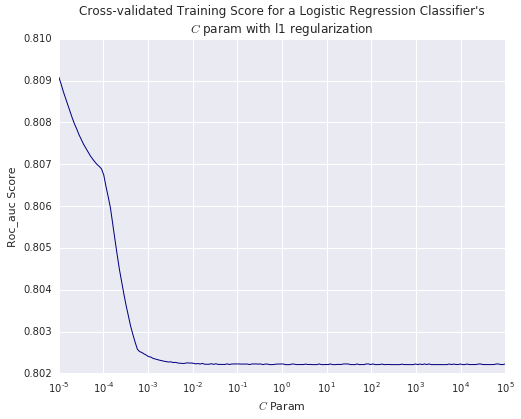
\includegraphics[width=1\linewidth]{figures/cross_validation/logreg_cv_regularization_l1_rocauc_series}
		\caption{CV mean average scores of the ``ROC AUC'' metric for \cref{target1}. The $l1$ regularization method on a logistic classifier was tested, varying along the $C$ hyperparameter.}
		\label{fig:rocauc_logreg_cv_l1_regularized_comparison}
	\end{center}
\end{figure}



\begin{figure}[h!]
	\begin{center}
		 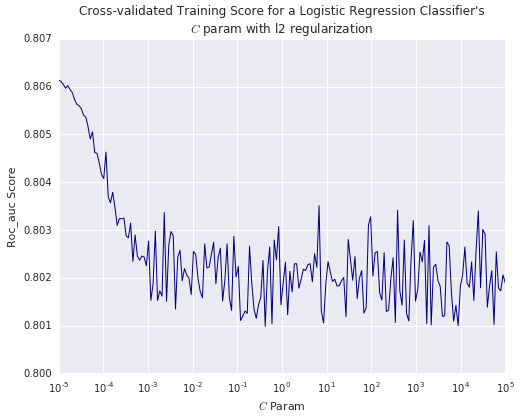
\includegraphics[width=1\linewidth]{figures/cross_validation/logreg_cv_regularization_l2_rocauc_series}
		\caption{CV mean average scores of the ``ROC AUC'' metric for \cref{target1}.  The $l2$ regularization method on a logistic classifier was tested, varying along the $C$ hyperparameter.}
		\label{fig:rocauc_logreg_cv_l2_regularized_comparison}
	\end{center}
\end{figure}


With these experiments we give an extended overview of how a complete model-selection pipeline is defined and we give examples of how we must iterate and evaluate different hyper-parameter configurations by scoring the cross-validated learners.
